% !TEX TS-program = pdflatex
% !TEX encoding = UTF-8 Unicode

% This is a simple template for a LaTeX document using the "article" class.
% See "book", "report", "letter" for other types of document.

\documentclass[10pt]{article} % use larger type; default would be 10pt
\usepackage{graphicx}
\usepackage{float}
\usepackage{caption}
\usepackage[utf8]{inputenc} % set input encoding (not needed with XeLaTeX)
\usepackage{amsmath,amsthm,amsfonts}
\usepackage{mathabx}
\usepackage{graphicx}
\usepackage{algorithm}
\usepackage{algorithmic}
\usepackage{hyperref}
\usepackage{listings}
\usepackage{textcomp}
%%% Examples of Article customizations
% These packages are optional, depending whether you want the features they provide.
% See the LaTeX Companion or other references for full information.

%For improved new command:
%(defining macros)
\usepackage{xparse}
%An example with optinal commands.
\NewDocumentCommand\optmin{mgg}%
{\begin{align*}
\text{minimize}&\quad {#1}\IfNoValueTF{#2}{}{\\
\text{subject to}&\quad {#2}}\IfNoValueTF{#3}{}{\\&\quad {#3}}
\end{align*}
}

%%% PAGE DIMENSIONS
\usepackage{geometry} % to change the page dimensions
\geometry{letterpaper} % or letterpaper (US) or a5paper or....
% \geometry{margin=2in} % for example, change the margins to 2 inches all round
% \geometry{landscape} % set up the page for landscape
%   read geometry.pdf for detailed page layout information

\usepackage{graphicx} % support the \includegraphics command and options
% \usepackage[parfill]{parskip} % Activate to begin paragraphs with an empty line rather than an indent

%%% PACKAGES
\usepackage{booktabs} % for much better looking tables
\usepackage{array} % for better arrays (eg matrices) in maths
\usepackage[section]{placeins} % With FloatBarrier control float
\usepackage{paralist} % very flexible & customisable lists (eg. enumerate/itemize, etc.)
\usepackage{verbatim}
%Setup listing for better matlab code display
\usepackage{listings}
\usepackage{color}
\usepackage{textcomp}
\definecolor{listinggray}{gray}{0.9}
\definecolor{lbcolor}{rgb}{0.9,0.9,0.9}
\lstset{
	backgroundcolor=\color{lbcolor},
	tabsize=4,
	rulecolor=,
	language=c++,
        basicstyle=\scriptsize,
        upquote=true,
        aboveskip={1.5\baselineskip},
        columns=fixed,
        showstringspaces=false,
        extendedchars=true,
        breaklines=true,
        prebreak = \raisebox{0ex}[0ex][0ex]{\ensuremath{\hookleftarrow}},
        frame=single,
        showtabs=false,
        showspaces=false,
        showstringspaces=false,
        identifierstyle=\ttfamily,
        keywordstyle=\color[rgb]{0,0,1},
        commentstyle=\color[rgb]{0.133,0.545,0.133},
        stringstyle=\color[rgb]{0.627,0.126,0.941},
}
% adds environment for commenting out blocks of text & for better verbatim
\usepackage{subfig} % make it possible to include more than one captioned figure/table in a single float
% These packages are all incorporated in the memoir class to one degree or another...

%%% HEADERS & FOOTERS
\usepackage{fancyhdr} % This should be set AFTER setting up the page geometry
\pagestyle{plain} % options: empty , plain , fancy
\renewcommand{\headrulewidth}{0pt} % customise the layout...
\lhead{}\chead{}\rhead{}
\lfoot{}\cfoot{\thepage}\rfoot{}

%%% SECTION TITLE APPEARANCE
\usepackage{sectsty}
\allsectionsfont{\sffamily\mdseries\upshape} % (See the fntguide.pdf for font help)
% (This matches ConTeXt defaults)

%%% ToC (table of contents) APPEARANCE
\usepackage[nottoc,notlof,notlot]{tocbibind} % Put the bibliography in the ToC
\usepackage[titles,subfigure]{tocloft} % Alter the style of the Table of Contents
\usepackage{tikz}
\usetikzlibrary{arrows}
\usetikzlibrary{calc}
\renewcommand{\cftsecfont}{\rmfamily\mdseries\upshape}
\renewcommand{\cftsecpagefont}{\rmfamily\mdseries\upshape} % No bold!

%%% shortcuts %%%
\newcommand{\heading}[1]{\vspace{1ex}\par\noindent{\bf #1}}
\def\immediateFigure#1{%
\smallskip\begin{center}#1\end{center}\smallskip }
\newcommand{\immfigw}[2] % immediate figure with prescribed width
{\immediateFigure{\mbox{\includegraphics[width=#2]{#1}}}}
\newcommand\eps{\varepsilon}
\newcommand*\colvec[3][]{
    \begin{bmatrix}\ifx\relax#1\relax\else#1\\\fi#2\\#3\end{bmatrix}
}
\newcommand\scalemath[2]{\scalebox{#1}{\mbox{\ensuremath{\displaystyle #2}}}}
\newcommand\vectt[1]{\boldsymbol{#1}}
\newcommand\inprod[2]{\langle{#1},{#2}\rangle}

%Shorthand for summation
\NewDocumentCommand\sumito{mmg}
{\sum_{\IfNoValueTF{#3}{i = 1}{i = {#3}}}^{#1}{#2}}
\NewDocumentCommand\sumjto{mmg}
{\sum_{\IfNoValueTF{#3}{j = 1}{j = {#3}}}^{#1}{#2}}
\NewDocumentCommand\sumkto{mmg}
{\sum_{\IfNoValueTF{#3}{k = 1}{k = {#3}}}^{#1}{#2}}
\NewDocumentCommand\sumlto{mmg}
{\sum_{\IfNoValueTF{#3}{l = 1}{l = {#3}}}^{#1}{#2}}

%%% END Article customizations
\newcommand\tsub[2]{{#1}_{\text{#2}}}
\newcommand\tsup[2]{{#1}^{\text{#2}}}
\newcommand\tspb[3]{{#1}^{\text{#2}}_{\text{#3}}}
\newcommand\RR{\mathbb{R}}
\newcommand\iprod[2]{\langle{#1},{#2}\rangle}
%%%Generates program flow chart using tikz
\usepackage{tikz}
\usetikzlibrary{shapes,arrows,positioning}
\tikzstyle{decision} = [diamond, draw, fill=blue!20, 
    text width=6em, text badly centered, node distance=3cm, inner sep=0pt]
\tikzstyle{block} = [rectangle, draw, fill=blue!20, 
    text width=8em, text centered, rounded corners, minimum height=4em]
\tikzstyle{line} = [draw, -latex']
\tikzstyle{cloud} = [draw, ellipse,fill=red!20, node distance=3cm,
    minimum height=2em]
%%%Commands below for this specific document only
\newcommand\infnorm[1]{\|{#1}\|_\infty}
\newcommand\set[1]{\left\{{#1}\right\}}
\NewDocumentCommand\norm{mg}
{\|{#1}\|\IfNoValueTF{#2}{}{_{#2}}}
\newcommand\cunit{C([0,1])}
\DeclareMathOperator{\tr}{tr}
\DeclareMathOperator*{\argmin}{argmin}
\newcommand\bSigma{\mathbf{\Sigma}}
\newcommand\bx{\mathbf{x}}
\newcommand\bv{\mathbf{v}}
\newcommand\bK{\mathbf{K}}
\newcommand\bJ{\mathbf{J}}
\newcommand\bM{\mathbf{M}}
%%% The "real" document content comes below...

\title{Appendix A: user manual for the particle method library}

\author{\sc Ningyuan WANG\\Daniel FORGER
}

\begin{document}
\setlength{\parindent}{0pt}
\maketitle

\section{Building and running the example program with Hodgkin-Huxley model}
\subsection{Structure of the repository}
This repository contains the source code for the method, in the form of a \texttt{C++} library, that consists of \texttt{particle\_method.h} and \texttt{particle\_method.cpp}, as well as an example program, which serves as a suggestion on how the library can be used. The example can be viewed by opening the \texttt{minimal\_HH\_mat\_example.sln} solution file.
The code is written using \texttt{C++}, and the example program is built on a \texttt{Windows} machine using \texttt{Microsoft Visual studio 2019}. The instruction will be based on this environment though the principle for building this program on other platform is similar. Since this program uses external libraries, some patience is needed in setting the program to work.
\subsection{Required external libraries}
The list of required libraries are listed according the specific header and source file loaded. 
\begin{itemize}
\item
\texttt{particle\_method.h} and \texttt{particle\_method.cpp}

There are two options for building these files. If macro \texttt{MATLAB\_VISUALIZE} is enabled, then \texttt{matlab} is required, and \texttt{libeng.lib;libmx.lib;libmat.lib;} are library files needed to be added at \texttt{Linker\textrightarrow Input\textrightarrow Additional dependencies} in the project property pages. Please refer to \href{www.mathworks.com/matlabcentral/answers/406574-how-can-i-compile-a-c-program-that-uses-matlab-engine-c-api-in-visual-studio-2017}{this page from mathworks website} for further instruction. Additonally, the system environment \texttt{MATLAB} should be set to the \texttt{matlab} root folder.

Alternatively, when real-time visualization is not required and the use of a large program is not preferred, the \texttt{HDF5} serves as an alternative data input output library. We recommend using \texttt{vcpkg} to setup \texttt{HDF5} library in visual studio. The following command
\begin{lstlisting}
vcpkg install hdf5[cpp]:x64-windows --recurse
\end{lstlisting}
  would download this package. Be warned that \texttt{hdf5} and \texttt{matlab} have conflicting \texttt{dll} files, and it is important to check which \texttt{dll} file is loaded at runtime. If \texttt{vcpkg} is not used, then \texttt{zlib.lib;hdf5.lib;hdf5\_cpp.lib} needed to be added at \texttt{Linker\textrightarrow Input\textrightarrow Additional dependencies}

Independent of the two options, \texttt{intel-tbb} is required for parallel computing. Additionally, \texttt{boost} and \texttt{Eigen} are libraries required. The following command
\begin{lstlisting}
vcpkg install tbb:x64-windows --recurse
vcpkg install boost[boost-odeint]:x64-windows
vcpkg install boost[boost-ublas]:x64-windows
vcpkg install boost[boost-program-options]:x64-windows
vcpkg install eigen3:x64-windows
\end{lstlisting}

would set these libraries. If \texttt{vcpkg} is not used, \texttt{tbb.lib} needs to be added to \texttt{Linker\textrightarrow Input\textrightarrow Additional dependencies}.

\item
\texttt{minimal\_XX\_neuron\_example.cpp}

The \texttt{boost-program-options} is needed to compile this file. If \texttt{vcpkg} is not used, then the correct version of \texttt{libboost\_program\_options} needs to be added to \texttt{Linker\textrightarrow Input\textrightarrow Additional dependencies}.
\item
\texttt{set\_XX\_eqns.h}
This header file does not require additional library to build.
\end{itemize}
\subsection{Building the program}

The projects in the solution are set to use the \texttt{matlab} version out-of-box. The program should build with one click if the external libraries are correctly set.

\subsection{Common issues and solution}
\begin{itemize}
\item
\texttt{LNK2001} at build time. Likely due to libraries not setup correctly, which may occur either when library is missing, or different versions of the same library exist. Using \texttt{vcpkg} would reduce the chance of this happening than manually tracing each library.
\item
undefined reference to \texttt{some\_function} at \texttt{xx.dll} at run time. In addition to the common cause of not properly setting the correct version of \texttt{matlab}, this is also likely to be caused by a conflict in \texttt{dll} file. \texttt{HDF5} and \texttt{matlab} both comes with \texttt{hdf5.dll}, however they are not interchangeable. To make sure the correct \texttt{dll} is loaded, check if \texttt{hdf5.dll} exist in current directory or the \texttt{Windows\textbackslash System32} directory. Then, the order of the directories stored in system \texttt{PATH} variable would determine which \texttt{hdf5.dll} will be used.
\end{itemize}
\subsection{Running the example program}
The program uses \texttt{boost::program\_options} to parse options, and help info can be accessed using the \texttt{-h} option:
\begin{figure}[H]
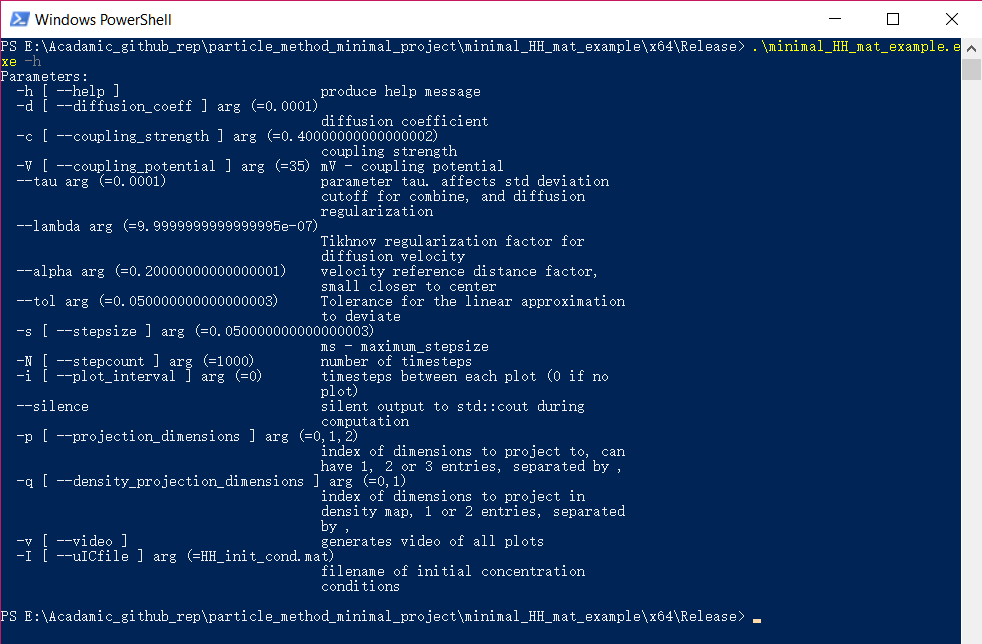
\includegraphics[width=\textwidth]{help_message}
\caption{Help message produced by the program}
\end{figure}

By default, the program will not produce any visual output as \texttt{-i (--plot\_interval) = 0}, and the only output files are \texttt{HHTestatend.mat}, which stores the end condition of the system as a linear combination of particles, and \texttt{coupling\_strength\_diff\_X\_coup\_Y.mat}, which logs the coupling strength, averaged membrane potential, and particle count through the process. 

Using the \texttt{-i \%d} option will generate a visualization that looks as follows: 
\begin{figure}[H]
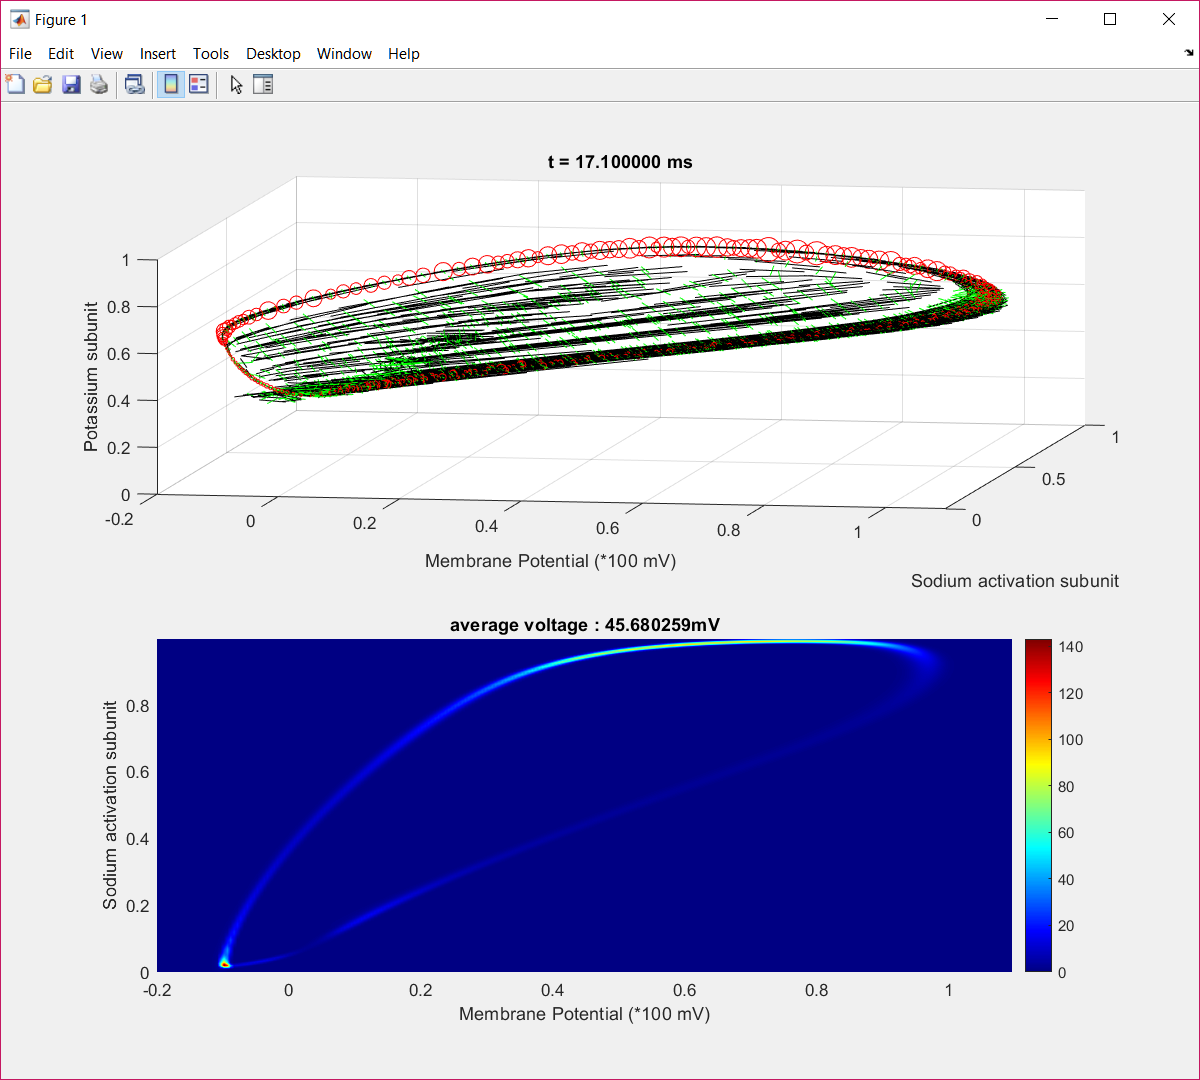
\includegraphics[width=\textwidth]{visualization_screenshot}
\caption{A screenshot of the visualization}
\end{figure}
Note that the plots, especially the density heat map is computationally intensive, and will significantly slow down the program. 
\section{Adapting the program to different problems}
The example program is called \emph{minimal} in the sense that only the most common parameters can be adjusted at run time, whereas the model and other parameters are determined at compile time, in order to present a short example. To adapt the program to a different model, the following areas needs to be considered: 
\subsection{Modifying models and parameters}
\label{str:Advdiffeqn}
In the example project, the models are contained in the \texttt{set\_hh\_eqns.h} and \texttt{set\_SAN\_eqns.h} for the Hodgkin-Huxley and Simplified averaged neuron model respectively. To set a model, a custom \texttt{struct Advection\_diffusion\_eqn} with the following properties needs to be defined:
\begin{lstlisting}
    vector_vector_function advection_velocity; //defines the time derivative of the system
    coupling_strength_function coupling_strength; //defines the strength of coupling output from a pre-synaptic neuron
    coupling_velocity_function coupling_velocity; // defines how a post-synaptic neuron is affected given a coupling input
    Matrix_type diffusion_coefficient; // a matrix-valued diffusion coefficient
    const index_type dimension; // Dimension of state space
    const bool state_variable_always_valid;// Is true when the state_variable can take any value as long as dimension is correct. Is false when the equation is only valid for a subset of the state space.
\end{lstlisting}
Additionally, if \texttt{state\_variable\_always\_valid} is false, then the following properties are also required:
\begin{lstlisting}
    vector_bool_function state_variable_in_domain;//Returns true if the variable is inside the domain.
    vector_vector_function state_variable_restrict_to_domain;//A method that maps particles out of domain back inside. (Such particles can be produced when particles are splitted.)
    //Note: Since a lambda function cannot change value of input
\end{lstlisting}
The following are two examples of \texttt{struct Advection\_diffusion\_eqn}.

The first example is the $2$-dimensional Van der Pol oscillator with that is coupled by the average value in the first variable:
\begin{lstlisting}
Advection_diffusion_eqn* set_van_der_pol_eqn(const value_type diffusion_coeff) {
    auto eqn_ptr = new Advection_diffusion_eqn(2, diffusion_coeff, true);//defines a 2-dimensional state space with an overloaded diffusion coefficient that is symmetric in each direction (i.e. diffusion coefficient matrix is identity matrix multiplied by scalar diffusion coefficient), and the state variable domain is the whole space.
    vector_vector_function advection_dynamics; //declares dynamics as a vector-valued function
    coupling_velocity_function coupling_velocity;//declares coupling velocity function (see example below)
    coupling_strength_function coupling_strength;//declares coupling strength function (see example below)
    //advection_dynamics is defined as the following lambda-function that returns the time derivative dxdt given the state variable x:
    advection_dynamics = [](const State_variable& x) {
        value_type mu = 1.5;
        State_variable dxdt(2);
        dxdt[0] = mu * (x[0] - pow(x[0], 3) / 3.0 - x[1]);
        dxdt[1] = x[0] / mu;
        return dxdt;
    };
    //A coupling velocity function takes input x as the state variable of the POST-synaptic oscillator, which given the vector-valued coupling_strength, will have its time derivative modified by dxdt:
    coupling_velocity = [](const State_variable& x, const value_type coupling_strength) {
        State_variable dxdt(2);
        dxdt[0] = coupling_strength;
        dxdt[1] = 0.0;
        return dxdt;//In this example, the dxdt is given by coupling_strength in the first coordinate.
    };
    //A coupling strength function computes the coupling strength output from a PRE-synaptic oscillator given its state in the current and a previous state, as well as the time difference between these two states.
    coupling_strength = [](const Particle& current_state, const Particle& prev_state, const value_type delta_t) {
        //NOTE: coupling strength should compute some average flow rate over the time_step period, NOT the instantaneous flow rate at a given time. 
        //The choice is made to avoid computing coupling strength on a derivative, 
        //which would be very sensitive to choice of timestep, and may miss some firing when time_step is too large. 
        //For an "averaged value type" coupling as shown here, this is not a big issue, but it does not hurt to compute average of the two. 
        const value_type coupling_coefficient = 0.5;
        return 0.5 * (current_state.center_location[0] + prev_state.center_location[0]) * coupling_coefficient * current_state.weight;//returns the average value in coordinate 1(defined by center_location) weighted with a coupling coefficient and the weight of this particle.
    };
    //NOTE: state_variable_in_domain and state_variable_restrict_to_domain not required since state variable is valid everywhere.
    //defines the return value using pointers. Due to constraint of C++, defining an incomplete class is only possible using pointers.
    eqn_ptr->advection_velocity = advection_dynamics;
    eqn_ptr->coupling_velocity = coupling_velocity;
    eqn_ptr->coupling_strength = coupling_strength;
    return eqn_ptr;
}
\end{lstlisting}
In the following example, the Hodgkin-Huxley equation with a threshold-type coupling is defined. It is copied from \texttt{set\_hh\_eqn.h} with additional comment:
\begin{lstlisting}
Advection_diffusion_eqn* set_Hodgkin_Huxley_eqn(const value_type diffusion_coeff, const value_type coupling_strength_coefficient, const value_type coupling_potential) {
    auto eqn_ptr = new Advection_diffusion_eqn(4, diffusion_coeff, false);//defines a 4-dimensional state space with an overloaded diffusion coefficient that is symmetric in each direction (i.e. diffusion coefficient matrix is identity matrix multiplied by scalar diffusion coefficient), and the state variable domain is restrained. (With restriction defined later)
    vector_vector_function advection_dynamics;
    coupling_velocity_function coupling_velocity;
    coupling_strength_function coupling_strength;
    //definition of a standard HH model: 
    advection_dynamics = [](const State_variable& x) {
        //x[0] = V / 100; rest ordered by M, N, H. 
        const value_type gna = 120;
        const value_type ena = 115; const value_type gk = 36;
        const value_type ek = -12;
        const value_type gl = 0.3;
        const value_type el = 10.613;
        const value_type appcurr = 8.0;
        State_variable dxdt(4U);
        value_type V = x[0] * 100.0;
        V += 1e-6 * (abs(V - 10.0)<5e-7 || abs(V - 25.0)<5e-7 || abs(V - 50.0)<5e-7);
        const value_type M = x[1];
        const value_type N = x[2];
        const value_type H = x[3];
        dxdt[0] = (appcurr + gna * M*M*M*H*(ena - V) + gk * (pow(N, 4))*(ek - V) + gl * (el - V)) / 100.0;
        //function y = Ah(V)
        const value_type Ah = 0.07*exp(-V / 20.0);
        //function y = Am(V)
        const value_type Am = (25.0 - V) / (10.0*(exp((25.0 - V) / 10.0) - 1.0));
        //function y = An(V)
        const value_type An = (10.0 - V) / (100.0*(exp((10.0 - V) / 10.0) - 1.0));
        //function y = Bh(V)
        const value_type Bh = 1.0 / (exp((30.0 - V) / 10.0) + 1.0);
        //function y = Bm(V)
        const value_type Bm = 4.0*exp(-V / 18.0);
        //function y = Bn(V)
        const value_type Bn = 0.125*exp(-V / 80.0);
        //%Bn = 0.125*exp(-V / 19.7); //this is for the Corrected HH model
        dxdt[1] = Am * (1 - M) - Bm * M;
        dxdt[2] = An * (1 - N) - Bn * N;
        dxdt[3] = Ah * (1 - H) - Bh * H;
        //std::cout << dxdt;
        return dxdt;
    };
    //definition of coupling strength, given PRE-synaptic oscillator particle at current state and a previous state that was coupling_time_step ago:
    coupling_strength = [coupling_strength_coefficient](const Particle& current_state, const Particle& prev_state, const value_type coupling_time_step) {
        //NOTE: coupling strength should compute the average flow rate over the coupling_time_step period, NOT the instantaneous flow rate at a given time. 
        //The choice is made to avoid computing coupling strength on a derivative, 
        //which would be very sensitive to choice of timestep, and may miss some firing when coupling_time_step is too large. 
        //For a "Threshold type" coupling, this means the value should be divided by coupling_time_step
        const value_type threshold_voltage = 0.45;// threshold voltage of 45 mV
        if (current_state.center_location[0] <= prev_state.center_location[0]) {
            //No coupling when the membrane potential is decreasing. 
            return 0.0;
        }
        //The following 3 lines compute the proportion (of the whole population) of the population crossing the threshold voltage:
        const value_type V_normalized = (current_state.center_location[0] - threshold_voltage) / sqrt(current_state.covariance_matrix(0,0));
        const value_type V_prev_normalized = (prev_state.center_location[0] - threshold_voltage) / sqrt(prev_state.covariance_matrix(0, 0));
        const value_type population_proportion = (erf(V_normalized / sqrt(2)) - erf(V_prev_normalized / sqrt(2)))*0.5;

        
        //Which is further adjusted by the coupling_strength_coefficient and weighr of particle, and divided by the time step since the coupling is computed as a velocity term, and should not be scaled by the choice of coupling time step.
        return population_proportion * coupling_strength_coefficient / coupling_time_step * current_state.weight;
    };
    const value_type coupling_potential_rescaled = coupling_potential / 100.0;
    //The coupling velocity defines how the POST-synaptic particle is affected, which in this particular example is a conductance-based coupling model:
    coupling_velocity = [coupling_potential_rescaled](const State_variable& target, const value_type coupling_strength) {
        //dV/dt = k(V_c - V) 
        State_variable rval(target.size());
        rval.fill(0.0);
        rval[0] = coupling_strength * (coupling_potential_rescaled - target[0]);
        return rval;
    };
    //Since HH model has 3 variables restricted between 0 and 1, the following function that determines if a coordinate is inside the domain is REQUIRED:
    vector_bool_function state_variable_in_domain;
    state_variable_in_domain = [](const State_variable x) {
        if (x[1]<0.0 || x[1] > 1.0 || x[2] < 0.0 || x[2] > 1.0 || x[3] < 0.0 || x[3] > 1.0)
            return false;
        return true;
    };
    //Additionally, a function to restrict such coordinates back to domain is also needed.
    vector_vector_function state_variable_restrict_to_domain;
    state_variable_restrict_to_domain = [](State_variable x) {
        auto x_copy = x;
        if (x_copy[1] < 0.0)
            x_copy[1] = 0.0;
        else if (x_copy[1] > 1.0)
            x_copy[1] = 1.0;
        if (x_copy[2] < 0.0)
            x_copy[2] = 0.0;
        else if (x_copy[2] > 1.0)
            x_copy[2] = 1.0;
        if (x_copy[3] < 0.0)
            x_copy[3] = 0.0;
        else if (x_copy[3] > 1.0)
            x_copy[3] = 1.0;
        return x_copy;
    };
    //define return value:
    eqn_ptr->advection_velocity = advection_dynamics;
    eqn_ptr->coupling_strength = coupling_strength;
    eqn_ptr->coupling_velocity = coupling_velocity;
    eqn_ptr->state_variable_in_domain = state_variable_in_domain;
    eqn_ptr->state_variable_restrict_to_domain = state_variable_restrict_to_domain;
    return eqn_ptr;
}
\end{lstlisting} 
\subsection{Modifying procedural source file}
After changing the model files, additional parameters independent from the model(such as timestep, total timestep count, and scalar parameters) needs modification as well. The procedural setup of the model in \texttt{main} and related functions also needs to be adjusted accordingly. How the desired parameters can be introduced is a generic programming problem and is beyond the scope here. However, we remind readers that:
\begin{itemize}
\item
Inside \texttt{run\_HH\_model}, make sure that the dimension are set correctly
\item
The plot parameters used here are specific to the chosen Hodgkin-Huxley model here
\end{itemize}
\subsection{Modifying initial condition}
The initial condition is defined by a \texttt{mat} file with following variables:
\begin{lstlisting}
%d-dimensional state variable, with initial condition as a linear combination of n particles:
w_array%1* n matrix, defines weight of each particle
x_array%d*n matrix, defines center location of each particle
sigma_array%d*d*n matrix, defines covariance of each particle
\end{lstlisting}
Note since \texttt{mat} uses column-major while \texttt{hdf5} uses row-major, the \texttt{h5} files will have reversed dimension ordering. An initial condition in \texttt{h5} file is defined as follows:
\begin{lstlisting}
//d-dimensional state variable, with initial condition as a linear combination of n particles:
x_array//n*d matrix of 64-bit floating-point
w_array//n*1 matrix of 64-bit floating-point
sigma_array//n*d*d matrix of 64-bit floating-point
\end{lstlisting}
\section{Usage for individual functions}
This section documents the usage of the functions and objects defined in \texttt{particle\_method.h}.
\begin{itemize}
\item
\texttt{\#define MATLAB\_VISUALIZE}: defines if the \texttt{matlab} version or \texttt{hdf5} version of data input/output should be used.
\item
Vector and Matrix-valued variables are defined as \texttt{Eigen} vectors and matrices. specifically: 
\begin{lstlisting}
typedef Eigen::VectorXd State_variable;
typedef Eigen::MatrixXd Matrix_type;
typedef double value_type;
typedef int index_type;
\end{lstlisting}
\item
Mathematical functions are defined using the lambda functions implemented using the \texttt{C++} standard library. Specifically: 
\begin{lstlisting}
typedef std::function<State_variable(const State_variable)> vector_vector_function;
typedef std::function<value_type(const State_variable)> vector_scalar_function;
typedef std::function<bool(const State_variable)> vector_bool_function;
typedef std::function<void(State_variable)> vector_void_function;
\end{lstlisting}
\item
\texttt{struct Particle} An asymmetric particle.
\begin{itemize}
\item
member variables

\begin{lstlisting}
	State_variable center_location;
	Matrix_type covariance_matrix;
	value_type weight;
\end{lstlisting}
\item
constructor

two initializing methods: 
\begin{lstlisting}
	Particle(index_type state_space_dimension = 1U) {
		weight = 0.0;
		center_location = Eigen::VectorXd::Zero(state_space_dimension);
		covariance_matrix = Eigen::MatrixXd::Identity(state_space_dimension, state_space_dimension);
	}
	Particle(const value_type weight, const State_variable& center_location, const Matrix_type& covariance_matrix) : weight(weight),center_location(center_location),covariance_matrix(covariance_matrix) {}
\end{lstlisting}

\item
helper functions:

method to find density values at a \texttt{location} in the state space: 
\begin{lstlisting}
value_type density_at(const State_variable& location) const;
\end{lstlisting}
Find density for marginal distribution where only a subset of coordinates in the \texttt{location} input is considered:
\begin{lstlisting}
value_type density_projection_at_coordinate(const State_variable& location, const std::vector<bool>& range_dimensions) const;//range_dimensions is of length dimension. e.g. TFTF means projection to dimension 0 and 2
\end{lstlisting}
\end{itemize}
\item
\texttt{struct Center\_level\_set}
This is a struct that is only used internally.
\item
\texttt{struct Adcection\_diffusion\_eqn} Refer to Section \ref{str:Advdiffeqn} for usage of member variables and functions. 
\item
\texttt{class Population\_density} The class containing the population density distribution, as a linear combination of particles it contained. 
\begin{itemize}
\item
Member variables:
\begin{lstlisting}
	const index_type dimension;
	//private: Note p_vect is not private only due to limit of tbb::concurrent_vector
	particle_vector p_vect;//container for the particles
\end{lstlisting}
where the \texttt{particle\_vector} is defined as follows:
\begin{lstlisting}
typedef tbb::concurrent_vector<Particle> particle_vector;
\end{lstlisting}
Note that \texttt{p\_vect} shall be treated as unavailable to access directly out side of the class scope, since the only reason for it to be not private is due to constraints of the \texttt{tbb} library used. 
\item
Constructor

An empty \texttt{Population\_density} can be initialized by the following constructor
\begin{lstlisting}
	Population_density(const index_type state_space_dimension, const value_type tau = 0.01 / 4.0 / log(2.0), const value_type lambda = 1e-6, const value_type alpha = 0.2)
		: dimension(state_space_dimension), tau(tau), lambda(lambda),alpha(alpha) {}
\end{lstlisting}

\item 
Container-related methods:
\texttt{Population\_density} can be accessed and modified like a vector, with \texttt{operater []}, \texttt{begin()}, \texttt{end()}, \texttt{size()} \texttt{resize()} and iterators as standard vectors.

To add particles to the population, use \texttt{append} to push back particle into the population:
\begin{lstlisting}
	particle_vector::iterator append(const Particle& particle) {
		p_vect.push_back(particle);
		//p_vect.insert(end(), particle);
		return end();
	}
\end{lstlisting}
\item
Evaluation methods

Information about the population can be obtained by using the following functions:
\begin{lstlisting}
value_type density_at(const State_variable& location) const;//returns population density at location
	value_type density_projection_at_coordinate(const State_variable& location, const std::vector<bool>& range_dimensions) const;//range_dimensions is of length dimension. e.g. TFTF means projection to dimension 0 and 2
	std::vector<value_type> density_at(const std::vector<State_variable>& location) const;//returns population density at all points in the location vector
	std::vector<value_type> density_projection_at_coordinate(const std::vector<State_variable>& location, const std::vector<bool>& range_dimensions) const;//range_dimensions is of length dimension. e.g. TFTF means projection to dimension 0 and 2
	double average_in_index(const int coord_idx) const;//returns the average value for coordinate i. (e.g. in HH model, average_in_index(0) returns average membrane potential.
\end{lstlisting}
\item
Visualization methods

If the macro \texttt{MATLAB\_VISUALIZE} is enabled, then the following plot functions that uses matlab engine is available: 
\begin{lstlisting}
    Plot_handle plot_density(std::vector<bool> projection_dimensions, const value_type x_lb, const value_type x_ub, const value_type y_lb, const value_type y_ub, const char* imagesc_options = "") const;
    //Plot the marginal population density projected into the projection_dimensions. 
    //e.g.: in a 4-dimensional space, projection_dimensions=TFTF projects the marginal density into 1st and 3rd dimension. 
    //The projection can be into a 1-dimensional or 2-dimensional subspace 
    //x_lb, x_ub, y_lb, y_ub is the lower and bounds for the coordinates to project to. y_lb, y_ub is not used when projection is into a 1-dimensional subspace
    //imagesc_options passes additional parameters into the imagesc command of matlab.
    Plot_handle plot_density(const value_type x_lb, const value_type x_ub, const value_type y_lb, const value_type y_ub, const char* imagesc_options = "") const;
    //project into first 2 dimensions. 
    Plot_handle plot_density(const int projection_dimension, const value_type x_lb, const value_type x_ub, const char *imagesc_options) const;//project into 1 dimension
    //Plot Flags: 1 overwrite, 2 not plot second eigenvec, 4 not plot first eigenvec.
    Plot_handle plot(std::vector<bool> projection_dimensions, const char* plot_options = "", const int plot_flags = 1);
    Plot_handle plot(const char* plot_options = "", const int plot_flags = 1);//project into first 2 dimensions. 
    Plot_handle output_center_and_weight() const;
    Plot_handle copy_particle_to_matlab(const index_type i) const;//COPY single particle to matlab workspace
    void output_particle(const index_type i, const char output_filename[] = "particle.mat") const;//OUTPUT single particle to a mat file
\end{lstlisting}

\item
Data I/O methods:

Independent of whether macro \texttt{MATLAB\_VISUALIZE} is enabled or not, the following functions allows input and output of population density as linear combination of particles. Please refer to the end of section \ref{str:Advdiffeqn} for the format of the files. 
\begin{lstlisting}
	void output_all_particles(const char output_filename[] = "particles.mat") const;//OUTPUT particles to a mat or h5 file
	void input_all_particles(const char input_filename[] = "particles.mat");//INPUT particles to a mat or h5 file
\end{lstlisting}
\end{itemize}
\item
\texttt{class Population\_density\_with\_equation : public Population\_density} The class containing a population density, and an advection-diffusion equation, which is an inherited class from \texttt{Population\_density}. 
\begin{itemize}
\item
Additional member variables:
\begin{lstlisting}
	const value_type tau;
	//tau NOW only affect particle combination. Larger tau leads to less aggressive particle combination.
    const value_type lambda;//regulariztion factor
    const value_type alpha;//advection velocity relative distance. alpha small uses level set closer to center.
\end{lstlisting}
\item
Constructor:
\begin{lstlisting}
    Population_density_with_equation(const Advection_diffusion_eqn& adv_diff_eqn, const index_type state_space_dimension, const value_type tau = 0.01 / 4.0 / log(2.0), const value_type lambda = 1e-6, const value_type alpha = 0.2)
        : Population_density(state_space_dimension),adv_diff_eqn(adv_diff_eqn), tau(tau), lambda(lambda), alpha(alpha) {
        set_ODE(adv_diff_eqn);
    }
\end{lstlisting}
\item
Methods for updating population density for \texttt{timestep}:
\begin{lstlisting}
    void update_ODE_const(const value_type timestep, const index_type stepcount = 1);//Updates population density with fixed timestep
    void update_ODE_adaptive(const value_type timestep, const index_type stepcount = 1);//Update population density with variable timestep that is at most timestep
    void update_ODE_adaptive_split(const value_type coupling_timestep, const index_type stepcount, const value_type rel_error_bound);//Update population density with variable timestep that is at most timestep. Moreover, if particles are too large to be accurate, particles are splitted automatically
\end{lstlisting}
\item
Functions to split and combine particles: 
\begin{lstlisting}
    void split_particles(const value_type rel_error_bound = DEFAULT_SPLIT_REL_ERROR);//Split all particles that are too large. No need to call if using update_ODE_adaptive_split
    void combine_particles();//combine particles. Should be called between each update_ODE step
\end{lstlisting}
\item
Additional helper functions:
\begin{lstlisting}
void check_linear_approx(const int particle_index) const;//prints information about accuracy of local linear approximation
\end{lstlisting}

\end{itemize}

\end{itemize}
\end{document}